\documentclass[10pt]{article}

\usepackage[utf8]{inputenc}
\usepackage{amsmath}
\usepackage{amssymb}
\usepackage{amsthm}
\usepackage[english]{babel}
\usepackage{fullpage}
\usepackage{graphics}
\usepackage[colorlinks=true,citecolor=blue,linkcolor=blue]{hyperref}
\usepackage{natbib}
\usepackage{todonotes}

% autoref fix for Chapter
\addto\extrasenglish{%
  \renewcommand{\sectionautorefname}{Section}%
}

\newtheorem{proposition}{Proposition}
\newtheorem{lemma}[proposition]{Lemma}
\newtheorem{corollary}[proposition]{Corollary}
\newtheorem{theorem}[proposition]{Theorem}

\newcommand{\R}{\mathbb{R}}

\renewcommand{\P}{\mathcal{P}}
\newcommand{\U}{\mathcal{U}}
\newcommand{\X}{\mathcal{X}}
\newcommand{\indicator}[1]{\mathbf{1}\left[{#1}\right]}
\newcommand{\x}{\mathbf{x}}
\newcommand{\KL}[2]{D\left(#1 \middle\| #2 \right)}
\newcommand{\norm}[1]{\left\| #1 \right\|}
\newcommand{\ip}[2]{\left\langle #1, #2 \right\rangle}

\DeclareMathOperator{\argmin}{argmin}
\DeclareMathOperator{\err}{err}
\DeclareMathOperator{\Exp}{\mathbf{E}}
\DeclareMathOperator{\VC}{VC}

\newcommand{\todoBalazs}[1]{\todo[backgroundcolor=blue]{Balazs: #1}}
\newcommand{\todoDavid}[1]{\todo[backgroundcolor=green]{David: #1}}
\newcommand{\todoSasha}[1]{\todo[backgroundcolor=orange]{Sasha: #1}}

\begin{document}

\title{The information-theoretic value of unlabeled data in semi-supervised learning}
\author{Alexander Golovnev \and D\'avid P\'al \and Bal\'azs Sz\"or\'enyi}

\maketitle

\begin{abstract}
We show a separation of the number of labeled examples required between learning
\emph{with} and \emph{without} the knowledge of the distribution of the
unlabeled data. For the class of projections over the Boolean hypercube of
dimension $n$, we show a separation by $\Theta(\log n)$ multiplicative factor.
For the class of monotone disjunctions over the Boolean hypercube of dimension
$n$, we show a separation by $\Theta(n)$ multiplicative factor. For the class of
halfspaces over $\R^n$, we show a separation by  $\Theta(n/\log n)$
multiplicative factor.

Learning with the knowledge of the distribution (a.k.a. \emph{fixed-distribution
learning}) can be viewed as an idealized scenario of semi-supervised learning
where the number of unlabeled data points is so great that the unlabeled
distribution is known exactly. For this reason, we call the separation the
\emph{value of unlabeled data}.
\end{abstract}


\section{Introduction}

\cite{Hanneke-2016} showed that for any class $C$ of Vapnik-Chervonenkis
dimension $d$ there exists an algorithm that $\epsilon$-learns any target
function from $C$ under any distribution from $O\left(\frac{d +
\log(1/\delta)}{\epsilon}\right)$ labeled examples with probability at least
$1-\delta$. For this paper, it is important to stress that Hanneke's algorithm
does \emph{not} receive the distribution of unlabeled data as input. On the
other hand, \cite{Benedek-Itai-1991} showed that for any class $C$ and any
distribution there exists an algorithm that $\epsilon$-learns any target from
$C$ from $O \left( \frac{\log N_{\epsilon/2} + \log (1/\delta)}{\epsilon}\right)$
labeled examples with probability at least $1-\delta$ where $N_{\epsilon/2}$ is the
size of an $\frac{\epsilon}{2}$-cover of $C$ with respect to the disagreement metric
$d(f,g) = \Pr[f(x) \neq g(x)]$. Here, it is important to note that Benedek-Itai
construct for each distribution a separate algorithm. In other words, they
construct a family of algorithms indexed by the (uncountably many) distributions
over the domain. Alternatively, we can think of Benedek-Itai's family of
algorithms as a single algorithm that receives the distribution as an input. It
is known that $N_\epsilon = O(1/\epsilon)^{O(d)}$; see \cite{Dudley-1978}. Thus,
ignoring $\log(1/\epsilon)$ factor, Benedek-Itai bound is never worse than
Hanneke's bound.

As we already mentioned, Benedek-Itai's algorithm receives as input the
distribution of unlabeled data. The algorithm uses it to construct an
$\frac{\epsilon}{2}$-cover. Unsurprisingly, there exist distributions which have
a small $\frac{\epsilon}{2}$-cover and thus sample complexity of Benedek-Itai's
algorithm on such distributions is significantly lower then the Hanneke's bound.
For instance, a distribution concentrated on a single point has an
$\frac{\epsilon}{2}$-cover of size $2$ for any positive $\epsilon$.

However, an algorithm does not need to receive the unlabeled distribution in
order to enjoy low sample complexity. For example, empirical risk minimization
(ERM) algorithm needs significantly less labeled examples to learn any target
under some unlabeled distributions. For instance, if a distribution is
concentrated on a single point, ERM needs only one labeled example to learn it.
One could be lead to believe that there exists an algorithm that does \emph{not}
receive the unlabeled distribution as input and achieves Benedek-Itai bound (or
a slightly worse bound) for \emph{every} distribution. In fact, one could think
that empirical risk minimization (ERM) or Hanneke's algorithm could be such
algorithm. If ERM, Hanneke's algorithm, or some other distribution-independent
algorithm had sample complexity that matches (or nearly matches) the optimal
distribution-specific sample complexity for \emph{every} distribution, we could
conclude that the knowledge of unlabeled data distribution is completely
useless.

As \cite{Darnstadt-Simon-Szorenyi-2013} showed this not the case. They showed
that \emph{any} algorithm for learning projections over $\{0,1\}^n$ that does
not receive the unlabeled distribution as input, requires, for some data
unlabeled distributions, more labeled examples than the Benedek-Itai bound.
However, they did not quantify this gap, beside stating that it grows without
bound as $n$ goes to infinity.

In this paper, we quantify the gap by showing that \emph{any}
distribution-independent algorithm for learning the class of projections over
$\{0,1\}^n$ requires, for some unlabeled distributions, $\Omega(\log n)$ times
as many labeled examples as Benedek-Itai bound. Furthermore, we show similar
results for the class of monotone disjunctions over the Boolean hypercube
$\{0,1\}^n$ where we show that any distribution-independent algorithm requires,
for some distributions, $\Omega(n)$ times as much labeled examples as the
Benedek-Itai bound. We show analogous result for halfspaces over $\R^n$, for
which we show that \emph{any} distribution-independent algorithm requires for
some unlabeled distributions $\Omega(\frac{n}{\log n})$ times as many labeled
examples as the Benedek-Itai bound.

\cite{Darnstadt-Simon-Szorenyi-2013} showed the gap for any class with
Vapnik-Chervonenkis dimension $d$ is at most $O(d)$. It is well known that
Vapnik-Chervonenkis dimensions of projections over $\{0,1\}^n$, monotone
disjunctions over $\{0,1\}^n$ and halfspaces over $\R^n$ are $\Theta(\log n)$,
$\Theta(n)$ and $\Theta(n)$ respectively. Thus our lower bounds match or almost
match the upper bound $O(d)$. However, it remains an open problem to close the
mismatch between $\Omega(\frac{n}{\log n})$ lower bound and $O(n)$ upper bound
for halfspaces over $\R^n$.

To better understand the relationship of the upper and lower bounds, we
illustrate the situation for the class of projections over $\{0,1\}^n$ in
Figure~\ref{figure:sample-complexity}. Recall that Vapnik-Chervonenkis dimension
of projections over $\{0,1\}^n$ is $\lfloor \log_2 n \rfloor$. This is a
folklore result, which we re-prove as
Proposition~\ref{proposition:vc-dimension-projections}.

\begin{figure}
\centering
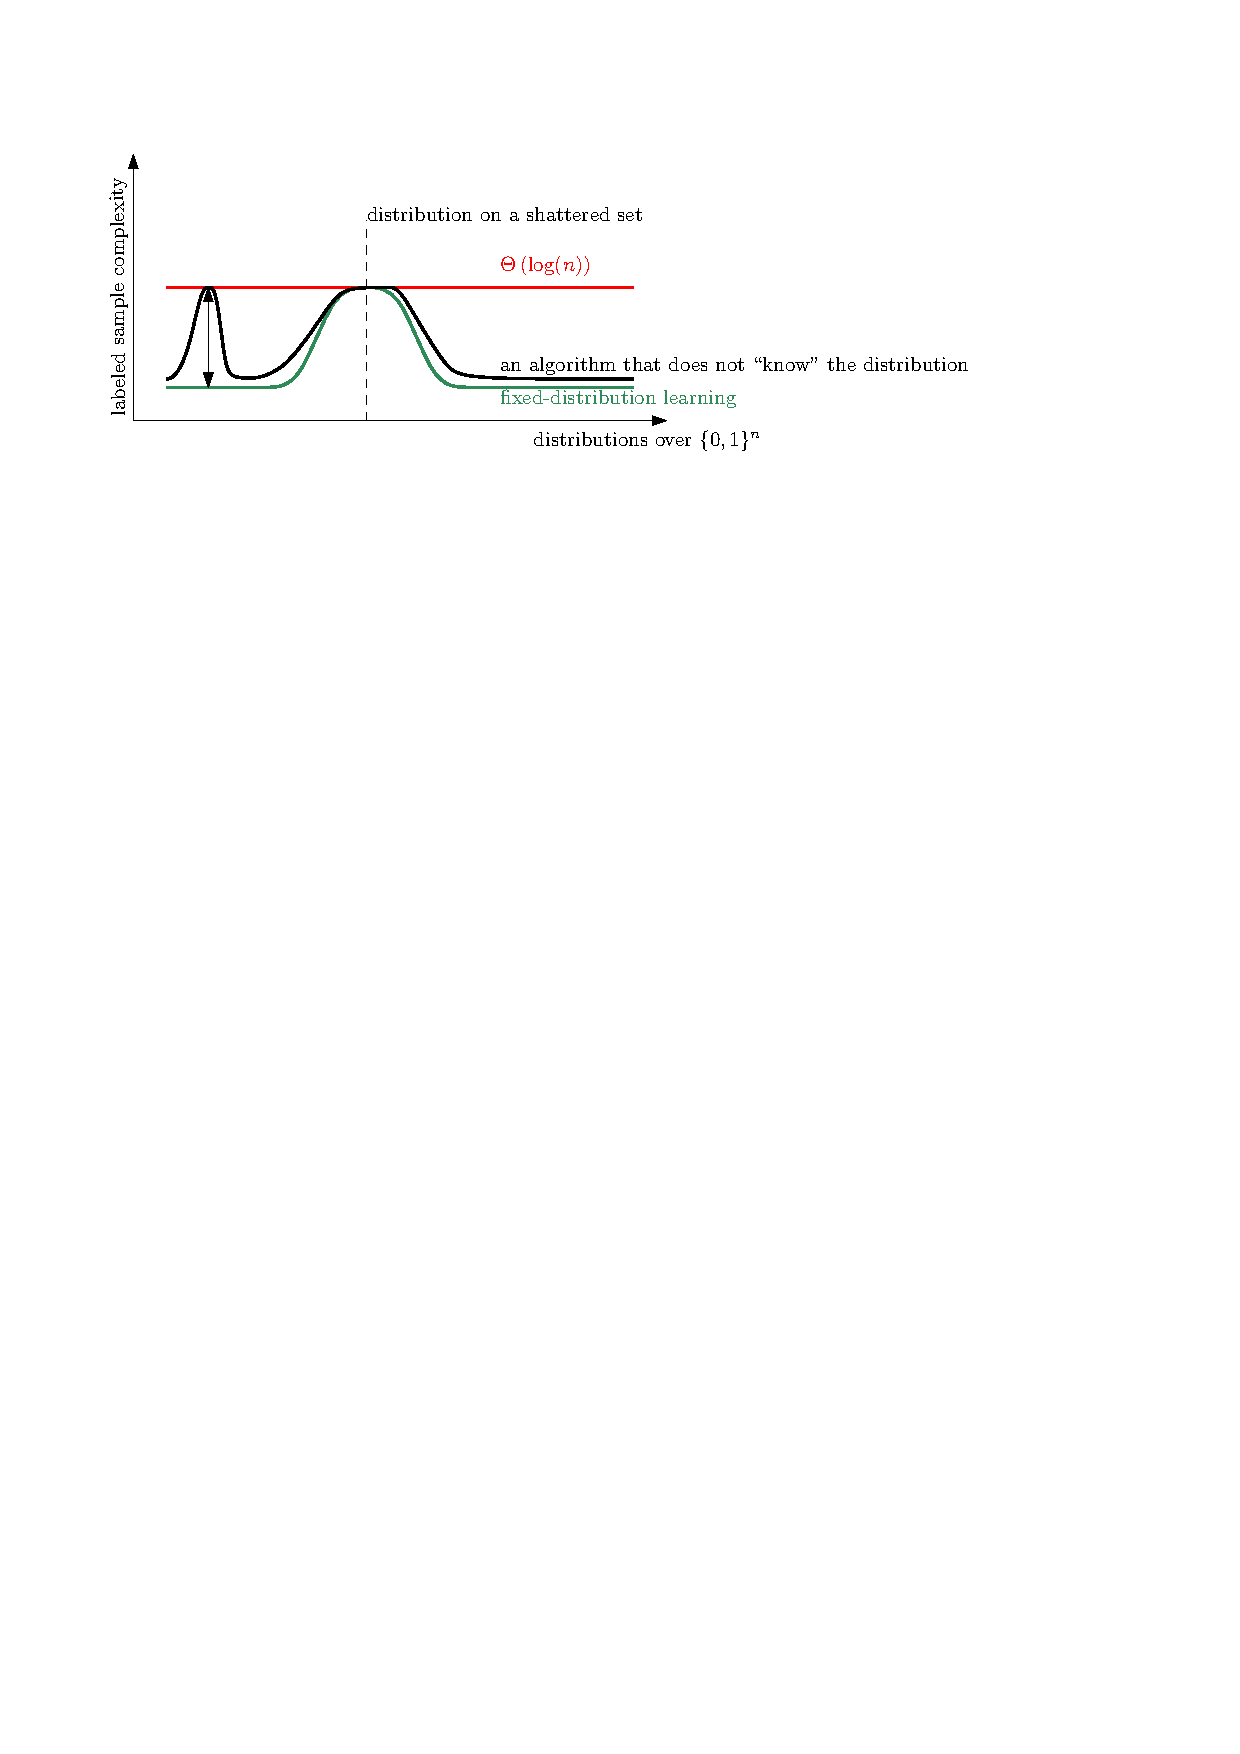
\includegraphics{figure}
\caption{\small The graph shows sample complexity bounds of learning a class of
projections over the domain $\{0,1\}^n$ under various unlabeled distributions.
We assume that $\epsilon$ and $\delta$ are constant, say, $\epsilon = \delta =
\frac{1}{10}$. The graph shows three lines. The red horizontal line is
Hanneke's bound for the class of projections, which is $\Theta(\VC(C_n)) =
\Theta(\log n)$. The green line is the Benedek-Itai bound. The green
line touches the red line for certain distributions, but is lower for other
distributions. In particular, for certain distributions the green line is
$O(1)$. The dashed line corresponds to a particular distribution on a shattered
set. This is where the green line and red line touch. Furthermore, here the
upper bound coincides with the lower bound for that particular distribution. The
black line is the sample complexity of an arbitrary
\emph{distribution-independent} algorithm. For example, the reader can think of
the ERM or Hanneke's algorithm.
We prove that there exist a distribution where the black line is
$\Omega(\log n)$ times higher than the green line. This separation is indicated
by the double arrow.}
\label{figure:sample-complexity}
\end{figure}

The paper is organized as follows. In \autoref{section:related-work} we review
prior work. \autoref{section:preliminaries} gives the necessary definitions and
basic probabilistic tools. Sections \ref{section:projections},
\ref{section:monotone-dijsunctions}, \ref{section:halfspaces} prove the
separation results for projections, monotone disjunctions, and halfspaces,
respectively. For completeness, in \autoref{section:epsilon-cover} we give a
proof of a simple upper bound $(e/\epsilon)^d$ on the size of the minimum
$\epsilon$-cover, and in \autoref{section:fixed-distribution-learning}, we re-prove
Benedek-Itai's $O \left( \frac{\log N_{\epsilon/2} + \log
(1/\delta)}{\epsilon}\right)$ sample complexity upper bound.

The proof technique in Sections \ref{section:projections}
\ref{section:monotone-dijsunctions}, \ref{section:halfspaces} is the same. The
differences only come up due to different combinatorial structure of the
three concept classes.

\section{Related Work}
\label{section:related-work}

The question of whether knowledge of unlabeled data distribution helps was
proposed and initially studied by \citet{Ben-David-Lu-Pal-2008}; see also
\citet{Lu-2009}. However, they considered only classes with Vapnik-Chervonenkis
dimension at most $1$, or classes with Vapnik-Chervonenkis dimension $d$ but
only distributions for which the size of the $\epsilon$-cover is
$\Theta(1/\epsilon)^{\Theta(d)}$, i.e. the $\epsilon$-cover is as large as it
can be.\footnote{For any concept class with Vapnik-Chervonenkis dimension $d$
and any distribution, the size of the smallest $\epsilon$-cover is at most
$O(1/\epsilon)^{O(d)}$. In fact, as we show in \autoref{section:epsilon-cover},
the size of the smallest $\epsilon$-cover is at most $(e/\epsilon)^d$.} In these
settings, for constant $\epsilon$ and $\delta$, the separation of labeled sample
complexities is at most a constant factor, which is exactly what
\citet{Ben-David-Lu-Pal-2008} proved. In these settings, unlabeled data are
indeed useless. However, these results say nothing about distributions with
$\epsilon$-cover of small size and it ignores the dependency on the
Vapnik-Chervonenkis dimension.

The question was studied in earnest by \citet{Darnstadt-Simon-Szorenyi-2013} who
showed two major results. First, they show that for any non-trivial concept
class $C$ and for every distribution, the ratio of the labeled sample
complexities between distribution-independent and distribution-dependent
algorithms is bounded by the Vapnik-Chervonenkis dimension. Second, they show
that for the class of projections over $\{0,1\}^n$, there are distributions
where the ratio grows to infinity as a function of $n$.

In learning theory, the disagreement metric and $\epsilon$-cover were introduced
by \citet{Benedek-Itai-1991} but the ideas are much older; see
e.g.~\citet{Dudley-1978, Dudley-1984}. The $O(1/\epsilon)^{O(d)}$ upper bound on
size of the smallest $\epsilon$-cover is by \citet[Lemma 7.13]{Dudley-1978}; see
also \citet[Chapter 4]{Devroye-Lugosi-2000} and \citet{Haussler-1995}.

For any distribution-independent algorithm and any class $C$ of
Vapnik-Chervonenkis dimension $d \ge 2$ and any $\epsilon \in (0,1)$ and $\delta
\in (0,1)$, there exists a distribution over the domain and a concept which
requires at least $\Omega \left(\frac{d + \log(1/\delta)}{\epsilon}\right)$
labeled examples to $\epsilon$-learn with probability at least $1 - \delta$;
see~\citet[Theorem 5.3]{Anthony-Bartlett-1999} and
\citet{Blumer-Ehrenfeucht-Haussler-Warmuth-1989,
Ehrenfeucht-Haussler-Kearns-Valiant-1989}. The proof of the lower bound
constructs a distribution that does \emph{not} depend on the algorithm. The
distribution is a particular distribution over a fixed set shattered by $C$. So
even an algorithm that knows the distribution requires $\Omega \left(\frac{d +
\log(1/\delta)}{\epsilon}\right)$ labeled examples.

\section{Preliminaries}
\label{section:preliminaries}

Let $\X$ be a non-empty set. We denote by $\{0,1\}^\X$ the class of all
functions from $\X$ to $\{0,1\}$. A \emph{concept class over a domain $\X$} is a
subset $C \subseteq \{0,1\}^\X$. A \emph{labeled example} is a pair $(x,y) \in
\X \times \{0,1\}$.

A \emph{distribution-independent learning algorithm} is a function
$A:\bigcup_{m=0}^\infty \left(\X \times \{0,1\} \right)^m \to \{0,1\}^\X$. In
other words, the algorithm gets as input a sequence of labeled examples $(x_1,
y_1), (x_2, y_2), \dots, (x_m, y_m)$ and outputs a function from $\X$ to
$\{0,1\}$. We allow the algorithm to output function that does not belong to
$C$, i.e., the algorithm can be improper. A \emph{distribution-dependent
algorithm} is a function that maps any probability distribution over $\X$ to a
distribution-independent algorithm.

Let $P$ be a probability distribution over a domain $\X$. For any two functions
$f:\X \to \{0,1\}$, $g:\X \to \{0,1\}$ we define the disagreement pseudo-metric
$$
d_P(f,g) = \Pr_{X \sim P}[f(X) \neq g(X)] \; .
$$
Let $C$ be concept class over $\X$, let $c \in C$, let $\epsilon, \delta \in (0,1)$.
Let  $X_1, X_2, \dots, X_m$ be an i.i.d. sample from $P$. We define the corresponding
labeled sample $T = ((X_1, c(X_1)), (X_2, c(X_2)), \dots, (X_m, c(X_m)))$.
We say that an algorithm $A$, \emph{$\epsilon$-learns} target $c$ from $m$ samples
with probability at least $1 - \delta$ if
$$
\Pr \left[d_P(c,A(T)) \le \epsilon \right]  \ge 1 - \delta \; .
$$

We recall the standard definitions from learning theory. For any concept $c:\X
\to \{0,1\}$ and any $S \subseteq \X$ we define $\pi(c,S) = \{x \in S ~:~ c(x) =
1 \}$. In other words, $\pi(c,S)$ is the set of examples in $S$ which $c$ labels
$1$. A set $S \subseteq \X$ is \emph{shattered} by a concept class $C$ if for
any subset $S' \subseteq S$ there exists a classifier $c \in C$ such that
$\pi(c,S) = S'$. \emph{Vapnik-Chervonenkis dimension} of a concept class $C$ is
the size of the largest set $S \subseteq \X$ shattered by $C$. A subset $C'$ of
a concept class $C$ is an \emph{$\epsilon$-cover} of $C$ for a probability
distribution $P$ if for any $c \in C$ there exists $c' \in C'$ such that
$d_P(c,c') \le \epsilon$.

To prove our lower bounds we need three general probabilistic results. The first
one is the standard Hoeffding bound. The other two are simple and intuitive
propositions. The first proposition says that if average error $d_P(c,A(T))$ is
high, the algorithm fails to $\epsilon$-learn with high probability. The second
proposition says that the best algorithm for predicting a bit based on some side
information, is to compute conditional expectation of the bit and thresholds it
at $1/2$.

\begin{theorem}[Hoeffding bound]
Let $X_1, X_2, \dots, X_n$ be i.i.d. random variables that lie in interval
$[a,b]$ with probability one and let $p=\frac{1}{n}\sum_{i=1}^n \Exp[X_i]$.
Then, for any $t \ge 0$,
$$
\Pr \left[{\frac {1}{n}} \sum_{i=1}^n X_i \ge p + t \right] \le e^{ - 2n t^2/(a-b)^2}  \qquad \text{and} \qquad
\Pr \left[{\frac {1}{n}} \sum_{i=1}^n X_i \le p - t \right] \le e^{ - 2n t^2/(a-b)^2}  \; . \\
$$
\end{theorem}

\begin{proposition}[Error probability vs. Expected error]
\label{proposition:error-probability-vs-expected-error}
Let $Z$ be a random variable such that $Z \le 1$ with probability one.
Then,
$$
\Pr[Z > t] \ge \frac{\Exp[Z] - t}{1 - t} \qquad \text{for any $t \in [0, 1)$.}
$$
\end{proposition}

\begin{proof}
We have
$$
\Exp[Z]
\le t \cdot \Pr[Z \le t] + 1 \cdot \Pr[Z > t]
= t \cdot (1 - \Pr[Z > t]) + \Pr[Z > t] \; .  \qquad \qedhere
$$
Solving for $\Pr[Z > t]$ finishes the proof.
\end{proof}

\begin{proposition}[Predicting Single Bit]
\label{proposition:single-bit}
Let $\U$ be a finite non-empty set. Let $U,V$ be random variables (possibly
correlated) such that $U \in \U$ and $V \in \{0,1\}$ with probability one. Let
$f:\U \to \{0,1\}$ be a predictor. Then,
$$
\Pr\left[ f(U) \neq V \right]
\ge \sum_{u \in \U} \left( \frac{1}{2} - \left| \frac{1}{2} -  \Exp \left[V \, \middle| \, U = u\right] \right| \right) \cdot \Pr[U = u] \; .
$$
\end{proposition}

\begin{proof}
We have
$$
\Pr \left[ f(U) \neq V \right] = \sum_{u \in \U} \Pr \left[ f(U) \neq V \, \middle| \, U = u \right] \cdot \Pr[U = u] \; .
$$
It remains to show that
$$
\Pr\left[ f(U) \neq V \, \middle| \, U = u \right]
\ge
\frac{1}{2} - \left| \frac{1}{2} -  \Exp \left[V \, \middle| \, U = u \right] \right| \; .
$$
Since if  $U=u$, the value $f(U) = f(u)$ is fixed, and hence
\begin{align*}
\Pr\left[ f(U) \neq V \, \middle| \, U = u \right]
& \ge \min\left\{ \Pr \left[ V = 1 \, \middle| \, U = u \right], \ \Pr \left[ V = 0 \, \middle| \, U = u \right] \right\} \\
& = \min\left\{ \Exp \left[ V  \, \middle| \, U = u \right], \ 1 - \Exp \left[ V \, \middle| \, U = u \right] \right\} \\
& = \frac{1}{2} - \left| \frac{1}{2} -  \Exp \left[ V  \, \middle| \, U = u \right] \right|
\end{align*}
We used the fact that $\min\{x, 1 - x\} = \frac{1}{2} - \left| \frac{1}{2} - x \right|$ for all $x \in \R$
which can be easily verified by considering two cases: $x \ge \frac{1}{2}$ and $x < \frac{1}{2}$.
\end{proof}

\section{Projections}
\label{section:projections}

In this section, we denote by $C_n$ the class of \emph{projections} over the
domain $\X = \{0,1\}^n$. The class $C_n$ consists of $n$ functions $c_1, c_2,
\dots, c_n$ from $\{0,1\}^n$ to $\{0,1\}$. For any $i \in \{1,2,\dots,n\}$, for
any $x \in \{0,1\}^n$, the function $c_i$ is defined as $c_i((x[1], x[2], \dots,
x[n])) = x[i]$.

For any $\epsilon \in (0,\frac{1}{2})$ and $n \ge 2$, we consider a family
$\P_{n,\epsilon}$ consisting of $n$ probability distributions $P_1, P_2, \dots,
P_n$ over the Boolean hypercube $\{0,1\}^n$. In order to describe the
distribution $P_i$, for some $i$, consider a random vector $X = (X[1], X[2],
\dots, X[n])$ drawn from $P_i$. The distribution $P_i$ is a product
distribution, i.e., $\Pr[X = x] = \prod_{j=1}^n \Pr[X[j] = x[j]]$ for any $x \in
\{0,1\}^n$. The marginal distributions of the coordinates are
$$
\Pr[X[j] = 1] =
\begin{cases}
\frac{1}{2} & \text{if $j = i$,} \\
\epsilon & \text{if $j\neq i$,} \\
\end{cases}
\qquad \text{for $j=1,2,\dots,n$.}
$$
The reader should think of $\epsilon$ as a constant that does not depend on $n$,
say, $\epsilon=\frac{1}{100}$.

\begin{proposition}
\label{proposition:vc-dimension-projections}
Vapnik-Chervonenkis dimension of $C_n$ is $\lfloor \log_2 n \rfloor$.
\end{proposition}

\begin{proof}
Let us denote the Vapnik-Chervonenkis dimension by $d$. Recall that $d$ is the
size of the largest shattered set. Let $S$ be any shattered set of size $d$.
Then, there must be at least $2^d$ distinct functions in $C_n$. Hence, $d \le
\log_2 |C_n| = \log_2 n$. Since $d$ is an integer, we conclude that $d \le
\lfloor \log_2 n \rfloor$.

On the other hand, we construct a shattered set of size $\lfloor \log_2 n
\rfloor$. The set will consists of points $x_1, x_2, \dots, x_{\lfloor \log_2 n
\rfloor} \in \{0,1\}^n$. For any $i \in \{1,2,\dots,\lfloor \log_2 n \rfloor\}$
and any $j \in \{0,1,2,\dots,n-1\}$, we define $x_i[j]$ to be the $i$-th bit
in the binary representation of the number $j$. (The bit at position $i=1$ is the
least significant bit.) It is not hard to see that for any $v \in
\{0,1\}^{\lfloor \log_2 n \rfloor}$, there exists $c \in C_n$ such that $v =
(c(x_1), c(x_2), \dots, c(x_{\lfloor \log_2 n \rfloor}))$. Indeed, given $v$,
let $k \in \{0,1,\dots,2^{\lfloor \log_2 n \rfloor} - 1\}$ be the number with
binary representation $v$, then we can take $c = c_{k+1}$.
\end{proof}


\begin{lemma}[Small cover]
Let $n \ge 2$ and $\epsilon \in (0,\frac{1}{2})$. Any distribution in $\P_{n,\epsilon}$
has $2\epsilon$-cover of size $2$.
\end{lemma}

\begin{proof}
Consider a distribution $P_i \in \P_{n,\epsilon}$ for some $i \in \{1,2,\dots,n\}$.
Let $j$ be an arbitrary index in $\{1,2,\dots,n\} \setminus \{i\}$.
Consider the projections $c_i, c_j \in C_n$. We claim that $C' = \{c_i, c_j\}$
is a $2\epsilon$-cover of $C_n$.

To see that $C'$ is a $2\epsilon$-cover of $C_n$, consider any $c_k \in C_n$.
We need to show that $d_{P_i}(c_i, c_k) \le 2\epsilon$ or $d_{P_i}(c_j, c_k)
\le 2\epsilon$. If $k = i$ or $k = j$, the condition is trivially satisfied.
Consider $k \in \{1,2,\dots,n\} \setminus \{i,j\}$. Let $X \sim P_i$. Then,
\begin{align*}
d_{P_i}(c_j, c_k)
& = \Pr[c_j(X) \neq c_k(X)] \\
& = \Pr[c_j(X) = 1 \wedge c_k(X) = 0] \\
  & \qquad + \Pr[c_j(X) = 0 \wedge c_k(X) = 1] \\
& = \Pr[X[j] = 1 \wedge X[k] = 0]  \\
  & \qquad + \Pr[X[j] = 0 \wedge X[k] = 1] \\
& = \Pr[X[j] = 1] \Pr[X[k] = 0] \\
  & \qquad + \Pr[X[j] = 0] \Pr[X[k] = 1] \\
& = 2 \epsilon \left( 1 - \epsilon \right)  \\
& < 2 \epsilon \; .
\end{align*}
\end{proof}

Using Bedek-Itai bound (Theorem~\ref{theorem:benedek-itai} in
\autoref{section:fixed-distribution-learning} in the supplementary material) we obtain the corollary below.
The corollary states that the distribution-dependent sample complexity
of learning target in $C_n$ under any distribution from $P_{n,\epsilon}$
does \emph{not} depend on $n$.

\begin{corollary}[Learning with knowledge of the distribution]
Let $n \ge 2$ and $\epsilon \in (0,\frac{1}{2})$.  There exists a
distribution-dependent algorithm such that for any distribution from $\P_{n,\epsilon}$,
any $\delta \in (0,1)$, any target function $c \in C_n$, if the algorithm gets
$$
m \ge \frac{12\ln(2/\delta)}{\epsilon}
$$
labeled examples, with
probability at least $1 - \delta$, it $4\epsilon$-learns the target.
\end{corollary}

The next theorem states that without knowing the distribution,
learning a target under a distribution from $\P_{n,\epsilon}$
requires at least $\Omega(\log n)$ labeled examples.

\begin{theorem}[Learning without knowledge of the distribution]
For any distribution-independent algorithm, any $\epsilon \in (0,\frac{1}{4})$ and any
$n \ge 600/\epsilon^3$ there exists a distribution $P \in \P_{n,\epsilon}$ and a target
concept $c \in C_n$ such that if the algorithm gets
$$
m \le \frac{\ln n}{3 \ln (1/\epsilon)}
$$
labeled examples, it fails to $\frac{1}{16}$-learn the target concept with probability
more than $\frac{1}{16}$.
\end{theorem}

\begin{proof}
Let $A$ be any learning algorithm. For ease of notation, we formalize it is a function
$$
A:\bigcup_{m=0}^\infty \left(\{0,1\}^{m \times n} \times \{0,1\}^m\right) \to \{0,1\}^{\{0,1\}^n} \; .
$$
The algorithm receives an $m \times n$ matrix and a binary vector of length $m$.
The rows of the matrix corresponds to unlabeled examples and the vector encodes
the labels. The output of $A$ is any function from $\{0,1\}^n \to \{0,1\}$.

We demonstrate the existence of a pair $(P,c) \in \P_{n,\epsilon} \times C_n$ which
cannot be learned with $m$ samples by the probabilistic method. Let $I$ be chosen
uniformly at random from $\{1,2,\dots,n\}$. We consider the distribution $P_I \in
\P_{n,\epsilon}$ and target $c_I \in C_n$. Let $X_1, X_2, \dots, X_m$ be an i.i.d.
sample from $P_I$ and let $Y_1 = c_I(X_1), Y_2 = c_I(X_2), \dots, Y_m =
c_I(X_m)$ be the target labels. Let $X$ be the $m \times n$ matrix with entries
$X_i[j]$ and let $Y = (Y_1, Y_2, \dots, Y_m)$ be the vector of labels. The
output of the algorithm is $A(X,Y)$. We will show that
\begin{equation}
\label{equation:projections-failure-probability}
\Exp \left[d_{P_I}(c_I, A(X,Y)) \right] \ge \frac{1}{8} \; .
\end{equation}
This means that there exists $i \in \{1,2,\dots,n\}$ such that
$$
\Exp \left[d_{P_i}(c_i, A(X,Y)) ~\middle|~ I = i \right] \ge \frac{1}{8} \; .
$$
By Proposition~\ref{proposition:error-probability-vs-expected-error},
$$
\Pr \left[ d_{P_i}(c_i, A(X,Y)) > \frac{1}{16} ~\middle|~ I = i \right] \ge \frac{\frac{1}{8} - \frac{1}{16}}{1 - \frac{1}{16}} > \frac{1}{16} \; .
$$

It remains to prove \eqref{equation:projections-failure-probability}. Let $Z$ be
a test sample drawn from $P_I$. That is, conditioned on $I$, the sequence $X_1,
X_2, \dots, X_m, Z$ is i.i.d. drawn from $P_I$. Then, by
Proposition~\ref{proposition:single-bit},
\begin{multline}
\label{equation:projections-expected-error-lower-bound}
\Exp \left[d_{P_I}(c_I, A(X,Y))\right]
= \Pr\left[ A(X,Y)(Z) \neq c_I(Z) \right] \ge \\
\sum_{\substack{x \in \{0,1\}^{m \times n} \\ y \in \{0,1\}^m \\ z \in \{0,1\}^n}} \left( \frac{1}{2} - \left| \frac{1}{2} - \Exp\left[ c_I(Z) \, \middle| \, X = x, Y = y, Z = z \right] \right| \right)
\\ \cdot \Pr \left[X = x, Y = y, Z = z \right]  \; .
\end{multline}
We need to compute $\Exp\left[ c_I(Z) \, \middle| \, X = x, Y = y, Z = z \right]$.
For that we need some additional notation.
For any matrix $x \in \{0,1\}^{m \times n}$, let $x[1], x[2], \dots, x[n]$ be its columns.
For any matrix $x \in \{0,1\}^{m \times n}$ and vector $y \in \{0,1\}^m$ let
$$
k(x,y) = \{ i \in \{1,2,\dots,n\} ~:~ x[i] = y \}
$$
be the set of indices of columns of $x$ equal to the vector $y$. Also, we define
$\norm{\cdot}$ to be the sum of absolute values of entries of a vector or a
matrix. (Since we use $\norm{\cdot}$ only for binary matrices and binary
vectors, it will be just the number of ones.)

For any $i \in \{1,2,\dots,n\}$,
\begin{multline*}
\Pr \left[I = i, X = x, Y = y \right] \\
=
\begin{cases}
\frac{1}{n} \left( \frac{1}{2} \right)^m \epsilon^{\norm{x} - \norm{y}} (1 - \epsilon)^{mn - \norm{x} + \norm{y}} & \text{if $i \in k(x,y)$.} \\
0 & \text{if $i \not \in k(x,y)$.} \\
\end{cases}
\end{multline*}
Therefore, for any $i \in \{1,2,\dots,n\}$,
\begin{align*}
& \Pr \left[I = i \, \middle| \, X = x, Y = y \right] \\
& \qquad = \frac{\Pr \left[I = i, X = x, Y = y \right]}{\Pr \left[ X = x, Y = y \right]} \\
& \qquad = \frac{\Pr \left[I = i, X = x, Y = y \right]}{\sum_{j \in k(x,y)} \Pr \left[ I = j, X = x, Y = y \right]} \\
& \qquad =
\begin{cases}
\frac{1}{|k(x,y)|} & \text{if $i \in k(x,y)$,} \\
0 & \text{if $i \not \in k(x,y)$,} \\
\end{cases}
\end{align*}

Conditioned on $I$, the variables $Z$ and $(X,Y)$ are independent. Thus,
for any $x \in \{0,1\}^n$, and $i = 1,2,\dots,n$,
\begin{align*}
& \Pr \left[Z = z \, \middle| \, I = i, X = x, Y = y \right] \\
& \qquad = \Pr \left[Z = z \, \middle| \, I = i \right] \\
& \qquad =
\begin{cases}
\frac{1}{2} \epsilon^{\norm{z} - 1} (1 - \epsilon)^{n - \norm{z}} & \text{if $z[i] = 1$,} \\
\frac{1}{2} \epsilon^{\norm{z}} (1 - \epsilon)^{n-1 - \norm{z}}& \text{if $z[i] = 0$.} \\
\end{cases}
\end{align*}
This allows us to compute the conditional probability
\begin{align*}
& \Pr \left[I = i, Z = z \, \middle| \, X = x, Y = y \right] \\
& \quad = \Pr \left[Z = z \, \middle| \, I = i, X = x, Y = y \right] \cdot \Pr \left[I = i \, \middle| \, X = x, Y = y \right] \\
& \quad =
\begin{cases}
\frac{1}{2|k(x,y)|} \epsilon^{\norm{z} - 1} (1 - \epsilon)^{n - \norm{z}} & \text{if $i \in k(x,y)$ and $z[i] = 1$,} \\
\frac{1}{2|k(x,y)|} \epsilon^{\norm{z}} (1 - \epsilon)^{n - 1 - \norm{z}} & \text{if $i \in k(x,y)$ and $z[i] = 0$,} \\
0 & \text{if $i \not \in k(x,y)$.} \\
\end{cases}
\end{align*}
For any $z \in \{0,1\}^n$, let
$$
s(x,y,z) = \{ i \in k(x,y) ~:~ z[i] = 1 \} \; ,
$$
and note that $s(x,y,z) \subseteq k(x,y)$.
Then,
\begin{align*}
& \Pr \left[Z = z \, \middle| \, X = x, Y = y \right] \\
& \quad = \sum_{i=1}^n \Pr \left[Z = z, I = i \, \middle| \, X = x, Y = y \right] \\
& \quad = \sum_{i \in k(x,y)} \Pr \left[Z = z, I = i \, \middle| \, X = x, Y = y \right] \\
& \quad = \sum_{i \in s(x,y,x)} \Pr \left[Z = z, I = i \, \middle| \, X = x, Y = y \right] \\
& \qquad + \sum_{i \in k(x,y) \setminus s(x,y,z)} \Pr \left[Z = z, I = i \, \middle| \, X = x, Y = y \right] \\
& \quad = \frac{1}{2|k(x,y)|} \cdot |s(x,y,z)| \cdot \epsilon^{\norm{z} - 1} (1 - \epsilon)^{n - \norm{z}} \\
& \qquad + \frac{1}{2|k(x,y)|} \cdot (|k(x,y)| - |s(x,y,z)|) \cdot \epsilon^{\norm{z}} (1 - \epsilon)^{n - 1 - \norm{z}} \\
& \quad = \frac{\epsilon^{\norm{z} - 1} (1 - \epsilon)^{n - 1 - \norm{z}}}{2|k(x,y)|} \cdot \left( |s(x,y,z)| \cdot (1 - 2\epsilon) + |k(x,y)| \cdot \epsilon \right) \; .
\end{align*}
Hence,
\begin{align*}
& \Exp\left[ c_I(Z) \, \middle| \, X = x, Y = y, Z = z \right] \\
& \quad = \Pr \left[ Z[I] = 1 \, \middle| \, X = x, Y = y, Z = z \right] \\
& \quad = \frac{\displaystyle \Pr \left[ Z[I] = 1, Z = z \, \middle| \, X = x, Y = y \right]}{\displaystyle \Pr \left[ Z = z \, \middle| \, X = x, Y = y \right]} \\
& \quad = \frac{\displaystyle \sum_{i=1}^n \Pr \left[ I = i, Z[i] = 1, Z = z \, \middle| \, X = x, Y = y \right]}{\displaystyle \Pr \left[ Z = z \, \middle| \, X = x, Y = y \right]} \\
& \quad = \frac{\displaystyle \frac{|s(x,y,z)|}{2|k(x,y)|} \cdot \epsilon^{\norm{z} - 1} (1 - \epsilon)^{n - \norm{z}}}{\displaystyle \frac{\epsilon^{\norm{z} - 1} (1 - \epsilon)^{n - 1 - \norm{z}}}{2|k(x,y)|}} \\
& \qquad \cdot \frac{1}{\left( |s(x,y,z)| \cdot (1 - 2\epsilon) + |k(x,y,z)| \cdot \epsilon \right) } \\
& \quad = \frac{\displaystyle |s(x,y,z)| \cdot (1 - \epsilon)}{\displaystyle |s(x,y,z)| \cdot (1 - 2\epsilon) + |k(x,y)| \cdot \epsilon } \\
& \quad = \frac{\displaystyle 1 - \epsilon}{\displaystyle 1 - 2\epsilon + \frac{|k(x,y)| \cdot \epsilon}{|s(x,y,z)|}} \\
\end{align*}

We now show that the last expression is close to $1/2$. It is easy to check that
$$
\frac{|k(x,y)| \cdot \epsilon}{|s(x,y,z)|} \in \left[\frac{5}{6}, 2 \right] \ \Rightarrow \ \frac{\displaystyle 1 - \epsilon}{\displaystyle 1 - 2\epsilon + \frac{|k(x,y)| \cdot \epsilon}{|s(x,y,z)|}} \in \left[ \frac{1}{4}, \frac{3}{4} \right].
$$
Indeed, since $\epsilon \in (0,\frac{1}{4})$,
$$
\frac{\displaystyle 1 - \epsilon}{\displaystyle 1 - 2\epsilon + \frac{|k(x,y)| \cdot \epsilon}{|s(x,y,z)|}} \ge
\frac{\displaystyle 1 - \epsilon}{\displaystyle 1 - 2\epsilon + 2} \ge \frac{\displaystyle 1 - 1/4}{\displaystyle 1 + 2} = \frac{1}{4}
$$
and
\begin{align*}
\frac{\displaystyle 1 - \epsilon}{\displaystyle 1 - 2\epsilon + \frac{|k(x,y)| \cdot \epsilon}{|s(x,y,z)|}}
& \le \frac{\displaystyle 1 - \epsilon}{\displaystyle 1 - 2\epsilon + 5/6} \\
& \le \frac{\displaystyle 1}{\displaystyle 1 - 1/2 + 5/6} = \frac{3}{4} \; .
\end{align*}
We now substitute this into the \eqref{equation:projections-expected-error-lower-bound}. We have
\begin{align*}
& \sum_{\substack{x \in \{0,1\}^{m \times n} \\ y \in \{0,1\}^m \\ z \in \{0,1\}^n}} \left( \frac{1}{2} - \left| \frac{1}{2} - \Exp\left[ c_I(Z) \, \middle| \, X = x, Y = y, Z = z \right] \right| \right) \\
& \qquad \qquad \qquad  \cdot \Pr \left[X = x, Y = y, Z = z \right] \\
& = \sum_{\substack{x \in \{0,1\}^{m \times n} \\ y \in \{0,1\}^m \\ z \in \{0,1\}^n}} \left( \frac{1}{2} - \left| \frac{1}{2} - \frac{\displaystyle 1 - \epsilon}{\displaystyle 1 - 2\epsilon + \frac{|k(x,y)| \cdot \epsilon}{|s(x,y,z)|}} \right| \right) \\
& \qquad \qquad \qquad  \cdot \Pr \left[X = x, Y = y, Z = z \right] \\
& \ge
\sum_{\substack{x \in \{0,1\}^{m \times n} \\ y \in \{0,1\}^m \\ z \in \{0,1\}^n \\ \frac{|k(x,y,z)| \epsilon}{|s(x,y,z)|} \in [\frac{5}{6},2]}} \left( \frac{1}{2} - \left| \frac{1}{2} - \frac{\displaystyle 1 - \epsilon}{\displaystyle 1 - 2\epsilon + \frac{|k(x,y)| \cdot \epsilon}{|s(x,y,z)|}} \right|  \right) \\
& \qquad \qquad \qquad  \cdot \Pr \left[X = x, Y = y, Z = z \right] \\
& \ge
\sum_{\substack{x \in \{0,1\}^{m \times n} \\ y \in \{0,1\}^m \\ z \in \{0,1\}^n \\ \frac{|k(x,y,z)| \epsilon}{|s(x,y,z)|} \in [\frac{5}{6},2]}} \left( \frac{1}{2} - \frac{1}{4} \right) \cdot \Pr \left[X = x, Y = y, Z = z \right] \\
& =
\frac{1}{4} \Pr \left[ \frac{|k(X,Y)| \cdot \epsilon}{|s(X,Y,Z)|} \in \left[\frac{5}{6}, 2 \right]  \right] \; .
\end{align*}
In order to prove \eqref{equation:projections-failure-probability}, we need to show that
$\frac{|k(X,Y)| \cdot \epsilon}{|s(X,Y,Z)|} \in \left[\frac{5}{6}, 2 \right]$ with
probability at least $1/2$. To that end, we define two additional random
variables
$$
K = |k(X,Y)| \qquad \text{and} \qquad S = |s(X,Y,Z)| \; .
$$
The condition $\frac{|k(X,Y)| \cdot \epsilon}{|s(X,Y,Z)|} \in \left[\frac{5}{6}, 2 \right]$ is equivalent to
\begin{equation}
\label{equation:ratio-condition}
\frac{1}{2} \epsilon \le \frac{S}{K} \le \frac{6}{5} \epsilon \; .
\end{equation}

First, we lower bound $K$. For any $y \in \{0,1\}^m$ and any $i,j \in \{1,2,\dots,n\}$,
\begin{align*}
& \Pr \left[ j \in k(X,Y)  \, \middle| \, Y = y, I = i \right] \\
& \qquad =
\begin{cases}
1 & \text{if $j = i$,} \\
\epsilon^{\norm{y}} (1 - \epsilon)^{m - \norm{y}} & \text{if $j \neq j$.}
\end{cases}
\end{align*}
Conditioned on $Y = y$ and $I=i$, the random variable $K - 1 = |k(X,Y) \setminus \{I\}|$ is
a sum of $n-1$ Bernoulli variables with parameter $\epsilon^{\norm{y}} (1 - \epsilon)^{m - \norm{y}}$, one for each column except for column $i$.
Hoeffding bound with $t = \epsilon^m/2$ and the loose lower bound $\epsilon^{\norm{y}} (1 - \epsilon)^{m - \norm{y}} \ge \epsilon^m$ gives
\begin{align*}
& \Pr \left[ \frac{K - 1}{n - 1} > \frac{\epsilon^m}{2}  \, \middle| \,  Y = y, I = i  \right] \\
& = \Pr \left[ \frac{K - 1}{n - 1} > \epsilon^m - t  \, \middle| \,  Y = y, I = i  \right] \\
& \ge \Pr \left[ \frac{K - 1}{n - 1} > \epsilon^{\norm{y}} (1 - \epsilon)^{m - \norm{y}} - t  \, \middle| \,  Y = y, I = i  \right] \\
& \ge 1 - e^{-2(n-1) t^2} \; .
\end{align*}
Since $m \le \frac{\ln n}{3 \ln (1/\epsilon)}$, we lower bound $t = \frac{\epsilon^m}{2}$ as
$$
t = \epsilon^m/2 > \frac{1}{2} \epsilon^\frac{\ln n}{3 \ln(1/\epsilon)} = \frac{1}{2\sqrt[3]{n}} \; .
$$
Since the lower bound is uniform for all choices of $y$ and $i$, we can remove
the conditioning and conclude that
$$
\Pr \left[ K > 1 + \frac{(n-1)}{2\sqrt[3]{n}} \right] \ge 1 - \exp \left(- \frac{(n-1)}{2 n^{2/3}} \right) \; .
$$
For $n \ge 25$, we can simplify it further to
$$
\Pr \left[ K \ge \frac{n^{2/3}}{2} \right] \ge \frac{3}{4} \; .
$$

Second, conditioned on $K=r$, the random variable $S$
is a sum of $r-1$ Bernoulli random variables with parameter $\epsilon$
and one Bernoulli random variable with parameter $1/2$. Hoeffding bound for any $t \ge 0$
gives that
\begin{align*}
\Pr \left[ \left| \frac{S}{K} - \frac{\epsilon(K - 1) + 1/2}{K} \right| < t \, \middle| \, K = r \right] \ge 1 - 2 e^{-2 r t^2} \; .
\end{align*}
Thus,
\begin{align*}
& \Pr \left[ \left| \frac{S}{K} - \frac{\epsilon(K - 1) + 1/2}{K} \right| < t \ \text{and} \ K \ge \frac{n^{2/3}}{2} \right] \\
& \ge \sum_{r = \lceil n^{2/3} / 2 \rceil}^n \Pr \left[ \left| \frac{S}{K} - \frac{\epsilon(K - 1) + 1/2}{K} \right| < t  \, \middle| \,  K = r \right] \\
& \qquad \qquad \qquad \qquad \cdot \Pr[K = r] \\
& \ge \sum_{r = \lceil n^{2/3} / 2 \rceil}^n \left( 1 - 2 e^{-2 r t^2} \right) \cdot \Pr[K = r] \\
& \ge \left( 1 - 2 e^{-n^{2/3}  t^2 / 2} \right) \cdot \Pr \left[ K \ge \frac{n^{2/3}}{2} \right] \; .
\end{align*}
We choose $t = \epsilon/4$. Since $n \ge 600/\epsilon^3$, we have $e^{-n^{2/3}  t^2 / 2} < \frac{1}{8}$ and thus
\begin{align*}
& \Pr \left[ \left| \frac{S}{K} - \frac{\epsilon(K - 1) + 1/2}{K} \right| < t \ \text{and} \ K \ge \frac{n^{2/3}}{2} \right] \\
& \qquad \ge \left( 1 - 2 e^{-n^{2/3}  t^2 / 2} \right) \cdot \Pr \left[ K \ge \frac{n^{2/3}}{2} \right] \\
& \qquad \ge \frac{3}{4} \left( 1 - 2 e^{-n^{2/3}  t^2 / 2} \right) \\
& \qquad > \frac{3}{4} \left( 1 - \frac{1}{4} \right) = \frac{9}{16} > \frac{1}{2} \; .
\end{align*}
We claim that $t = \epsilon/4$,
$\left| \frac{S}{K} - \frac{\epsilon(K - 1) + 1/2}{K} \right| < t$
and $K \ge \frac{n^{2/3}}{2}$ imply \eqref{equation:ratio-condition}.
To see that, note that $\left| \frac{S}{K} - \frac{\epsilon(K - 1) + 1/2}{K} \right| < t$ is equivalent to
$$
\frac{\epsilon(K - 1) + 1/2}{K} - t < \frac{S}{K} < \frac{\epsilon(K - 1) + 1/2}{K} + t
$$
which implies that
$$
p \left(1 - \frac{1}{K} \right) - t < \frac{S}{K} < \epsilon \left(1 - \frac{1}{K} \right) + \frac{1}{2K} + t \; .
$$
Since $K \ge \frac{n^{2/3}}{2}$ and $n \ge 25$ we have $K > 4$, which implies that
$$
\frac{3}{4} \epsilon - t < \frac{S}{K} < \frac{3}{4} \epsilon + \frac{1}{2K} + t \; .
$$
Since $K \ge \frac{n^{2/3}}{2}$ and $n \ge \frac{12}{\epsilon^{3/2}}$ we have $K > \frac{5}{2\epsilon}$, which implies that
$$
\frac{3}{4} \epsilon - t < \frac{S}{K} < \frac{3}{4} \epsilon + \frac{\epsilon}{5} + t \; .
$$
Since $t = \epsilon/4$, the condition \eqref{equation:ratio-condition} follows.
\end{proof}

\section{Monotone Disjunctions}
\label{section:monotone-dijsunctions}

In this section, we denote by $C_n$ the class of monotone disjunctions over the
Boolean hypercube $\X = \{0,1\}^n$. There are $2^n$ functions in $C_n$. For each
subset $I \subseteq \{1,2,\dots,n\}$ there is monotone disjunction $c_I:\X \to
\{0,1\}$ defined for any $x = (x[1],
x[2], \dots, x[n]) \in \X$ as
$$
c_I(x) = \bigvee_{i \in I} x[i] \; .
$$
If $I = \emptyset$, we define $c_I$ as the constant zero function.

For any even $n \ge 4$ and any $\epsilon \in (0,\frac{1}{2})$, we consider a
family of probability distributions $\P_{n,\epsilon}$ over the Boolean hypercube $\X =
\{0,1\}^n$. The family consists of $\binom{n}{n/2}$ probability distributions.
For each subset $J \subseteq \{1,2,\dots,n\}$ of size $|J| = n/2$
there is a probability distribution $P_J \in \P_{n,\epsilon}$. To describe a distribution $P_J$
for some $J \subseteq \{1,2,\dots,n\}$, consider a random vector $X = (X[1],
X[2], \dots, X[n])$ drawn from $P_J$. The distribution $P_J$ is a product
distribution, i.e., $\Pr[X=x] = \prod_{j=1}^n \Pr[X[j] = x[j]]$ for any $x \in
\{0,1\}^n$. The marginal distributions are
\begin{align*}
\Pr[X[j] = 1] =
\begin{cases}
1 - \sqrt[n/2 - 1]{1 - \epsilon}  & \text{if $j \in J$,} \\
1 - \epsilon & \text{if $j \not \in J$,}
\end{cases}
&& \text{for $j=1,2,\dots,n$.}
\end{align*}
Note that $1 - \sqrt[n/2-1]{1 - \epsilon} < \frac{1}{2}$ and $1 - \epsilon >
\frac{1}{2}$. Same as before, the reader should think of $\epsilon$ as a
constant that does not depend on $n$, say, $\epsilon=\frac{1}{100}$.

\begin{proposition}[Vapnik-Chervonenkis dimension]
Vapnik-Chervonenkis dimension of the class of monotone disjunctions $C_n$ is $n$.
\end{proposition}

\begin{proof}
Let us denote the Vapnik-Chervonenkis dimension by $d$. Recall that $d$ is the
size of the largest shattered set. Let $S$ be any shattered set of size $d$.
Then, there must be at least $2^d$ distinct functions in $C_n$. Hence, $d \le
\log_2 |C_n| = n$.

On the other hand, we construct a shattered set of size $n$. For any $i \in
\{1,2,\dots,n\}$, let $e_i = (0, \dots, 0, 1, 0, \dots, 0)$ be vector in
$\{0,1\}^n$ with all coordinate equal to zero except for the $i$-th coordinate
which is equal to $1$. We claim that the set $S = \{e_1, e_2, \dots, e_n\}$ is
shattered. For any binary vector $S' \subseteq S$, consider the set $I = \{ i
\in \{1,2,\dots,n\} ~:~ e_i \in S' \}$ and the monotone disjunction $c_I$. It is
not hard to see that $S' = \pi(c, S)$ since $c_I(e_i) = \indicator{i \in I} =
\indicator{e_i \in S'}$. Thus the set $\{e_1, e_2, \dots, e_n\}$ is shattered.
\end{proof}

\begin{lemma}
For any even $n \ge 4$, any $\epsilon \in (0,\frac{1}{2})$, and any distribution
from $\P_{n,\epsilon}$ there exists an $\epsilon$-cover of the class of monote
disjunctions $C_n$ of size $3$.
\end{lemma}

\begin{proof}
Let $J \subseteq \{1,2,\dots,n\}$ such that $|J| = n/2$ and let $P_J \in \P_{n,\epsilon}$.
Let $C' = \{c_J, c_\emptyset, c_{\{1,2,\dots,n\}}\}$.
We claim that $C'$ is an $\epsilon$-cover of $C_n$ under the distribution $P_J$.
Let $I \subseteq \{1,2,\dots,n\}$ be arbitrary and let $c_I \in C_n$ be the
corresponding disjunction. We need to show that $d_{P_J}(c_I, c_J) \le \epsilon$
or $d_{P_J}(c_I, c_\emptyset) \le \epsilon$ or $d_{P_J}(c_I,
c_{\{1,2,\dots,n\}}) \le \epsilon$. We consider three cases.

Case 1: $I = J$. Clearly, $d_{P_J}(c_I, c_J) = 0$.

Case 2: $I \subseteq J$ and $I \neq J$. We show that $d_{P_J}(c_I, c_\emptyset) \le \epsilon$.
Note that $|I| \le n/2 - 1$. Let $X \sim P_J$. Then,
\begin{align*}
d_{P_J}(c_I, c_\emptyset)
& = \Pr[c_I(X) \neq c_\emptyset(X)] \\
& = \Pr[c_I(X) = 1] \\
& = \Pr \left[ \bigvee_{i \in I} (X[i] = 1) \right] \\
& = 1 - \Pr \left[ \bigwedge_{i \in I} (X[i] = 0) \right] \\
& = 1 - \prod_{i \in I} \Pr \left[ X[i] = 0 \right] \\
& = 1 - \prod_{i \in I} \sqrt[n/2 - 1]{1 - \epsilon} \\
& \le 1 - \bigg( \sqrt[n/2-1]{1 - \epsilon} \bigg)^{n/2-1} \\
& = 1 - (1 - \epsilon) \\
& = \epsilon
\end{align*}

Case 3: If $I \not \subseteq J$. We show that $d_{P_J}(c_I, c_{\{1,2,\dots,n\}}) \le \epsilon$.
Since $I \not \subseteq J$, there exists $k \in I \setminus J$. Let $X \sim P_J$. Then,
\begin{align*}
d_{P_J}(c_I, c_{\{1,2,\dots,n\}})
& = \Pr [c_I(X) \neq c_{\{1,2,\dots,n\}}(X)] \\
& = \Pr [c_I(X) = 0 \ \text{and} \ c_{\{1,2,\dots,n\}}(X) = 1] \\
& \le  \Pr [c_I(X) = 0 ] \\
& = \Pr \left[ \bigwedge_{i \in I} (X[i] = 0) \right] \\
& = \prod_{i \in I} \Pr \left[ X[i] = 0 \right] \\
& \le \Pr \left[ X[k] = 0 \right] \\
& = \epsilon \; .
\end{align*}
\end{proof}

Using Bedek-Itai bound (Theorem~\ref{theorem:benedek-itai} in
\autoref{section:fixed-distribution-learning}) we obtain the corollary below.
The corollary states that the distribution-dependent sample complexity
of learning target in $C_n$ under any distribution from $P_{n,\epsilon}$
does \emph{not} depend on $n$.

\begin{corollary}[Learning with knowledge of the distribution]
Let $n \ge 4$ and $\epsilon \in (0,\frac{1}{2})$.  There exists a
distribution-dependent algorithm such that for any distribution from $\P_{n,\epsilon}$,
any $\delta \in (0,1)$, any target function $c \in C_n$, if the algorithm gets
$$
m \ge \frac{24\ln(3/\delta)}{\epsilon}
$$
labeled examples, with
probability at least $1 - \delta$, it $2\epsilon$-learns the target.
\end{corollary}

The next theorem states that without knowing the distribution,
learning a target under a distribution from $\P_{n,\epsilon}$
requires at least $\Omega(n)$ labeled examples.

\begin{theorem}[Learning without knowledge of the distribution]
For any distribution-independent algorithm, any $\epsilon \in (0,\frac{1}{4})$ and any
$n \ge ???$ there exists a distribution $P \in \P_{n,\epsilon}$ and a target
concept $c \in C_n$ such that if the algorithm gets
$$
m \le n ???
$$
labeled examples, it fails to $\frac{1}{16}$-learn the target concept with probability
more than $\frac{1}{16}$.
\end{theorem}

\begin{proof}
Let $A$ be any learning algorithm. For ease of notation, we formalize it is as a function
$$
A:\bigcup_{m=0}^\infty \left(\{0,1\}^{m \times n} \times \{0,1\}^m\right) \to \{0,1\}^{\{0,1\}^n} \; .
$$
The algorithm receives an $m \times n$ matrix and a binary vector of length $m$.
The rows of the matrix corresponds to unlabeled examples and the vector encodes
the labels. The output of the $A$ is any function from $\{0,1\}^n \to \{0,1\}$.

We demonstrate the existence of a pair $(P,c) \in \P_{n,\epsilon} \times C_n$
which cannot be learned with $m$ samples by probabilistic method. Let $E
\subseteq \{1,2,\dots,n\}$ be a random subset of size $n/2$. That is, $\Pr[E =
I] = 1/\binom{n}{n/2}$ for any fixed set $I \subseteq \{1,2,\dots,n\}$ of
size $n/2$. We consider distribution $P_E \in \P_{n,\epsilon}$ and target $c_E
\in C_n$. Let $X_1, X_2, \dots, X_m$ be an i.i.d. sample from $P_E$ and let $Y_1 =
c_E(X_1), Y_2 = c_E(X_2), \dots, Y_m = c_E(X_m)$ be the target labels. Let $X$
be the $m \times n$ matrix with entries $X_i[j]$ and let $Y = (Y_1, Y_2, \dots,
Y_m)$ be the vector of labels. The output of the algorithm is $A(X,Y)$. We will
show that
\begin{equation}
\label{equation:monotone-disjunctions-failure-probability}
\Exp \left[d_{P_E}(c_E, A(X,Y)) \right] \ge \frac{1}{8} \; .
\end{equation}
This means that there exists $I \subseteq \{1,2,\dots,n\}$ of size $|I|=n/2$ such that
$$
\Exp \left[d_{P_I}(c_I, A(X,Y)) ~\middle|~ E = I \right] \ge \frac{1}{8} \; .
$$
By Proposition~\ref{proposition:error-probability-vs-expected-error},
$$
\Pr \left[ d_{P_I}(c_I, A(X,Y)) > \frac{1}{16} ~\middle|~ E = I \right] \ge \frac{\frac{1}{8} - \frac{1}{16}}{1 - \frac{1}{16}} > \frac{1}{16} \; .
$$
It remains to prove \eqref{equation:monotone-disjunctions-failure-probability}.
Let $Z$ be a test sample drawn from $P_I$. That is, conditioned on $I$, the sequence $X_1, X_2, \dots, X_m, Z$ is i.i.d. drawn from $P_I$.
Then, by Proposition~\ref{proposition:single-bit},
\begin{multline}
\label{equation:monotone-disjuctions-xpected-error-lower-bound}
\Exp \left[d_{P_E}(c_E, A(X,Y))\right]
= \Pr\left[ A(X,Y)(Z) \neq c_E(Z) \right] \\
\ge \sum_{\substack{x \in \{0,1\}^{m \times n} \\ y \in \{0,1\}^m \\ z \in \{0,1\}^n}} \left( \frac{1}{2} - \left| \frac{1}{2} - \Exp\left[ c_E(Z) \, \middle| \, X = x, Y = y, Z = z \right] \right| \right) \cdot \Pr \left[X = x, Y = y, Z = z \right]  \; .
\end{multline}
We need to compute $\Exp\left[ c_E(Z) \, \middle| \, X = x, Y = y, Z = z \right]$.
\end{proof}


\subsection{Old Junk}

Consider a distribution $P_J \in \P_{n,p,p'}$. We compute the distance $d_P(c_I, c_{I'})$ between
any two monotone disjunctions $c_I$ and $c_{I'}$. For any subset $K \subseteq \{1,2,\dots,n\}$, let
$A_K$ be the event that all for all $i \in K$, $x_i = 0$.
\begin{align*}
d_P(c_I, c_J)
& = \Pr_{x \sim P}[c_I(x) \neq c_J(x)] \\
& = \Pr_{x \sim P}[A_{I \cap J} \wedge ((A_{I \setminus J} \wedge \overline{A_{J \setminus I}}) \vee (\overline{A_{I \setminus J}} \wedge A_{J \setminus I} )) ] \\
& = \Pr[A_{I \cap J}] \cdot \left\{ \Pr[A_{I \setminus J}] (1 - \Pr[A_{J \setminus I}]) + (1 - \Pr[A_{I \setminus J}]) \Pr[A_{J \setminus I}] \right\} \\
& = \Pr[A_{I \cap J}] \cdot \left\{ \Pr[A_{I \setminus J}] + \Pr[A_{J \setminus I}] - 2 \Pr[A_{I \setminus J}] \Pr[A_{J \setminus I}] \right\} \\
& = \Pr[A_I] + \Pr[A_J] - 2 \Pr[A_{I \cup J}] \\
& = \prod_{i \in I} (1 - p_i) + \prod_{j \in J} (1 - p_j) - 2 \prod_{k \in I \cup J} (1 - p_k) \; . \\
\end{align*}

\section{Halfspaces}
\label{section:halfspaces}

In this section, we denote by $C_n$ the class of halfspaces over $\X = \R^n$. There
are infinitely many functions in $C_n$. For every non-zero vector $w \in \R^n$, there is a half space
$$
c_w(x) = \indicator{\ip{w}{x} \ge 0} \qquad \qquad \text{for any $x \in \R^n$} \; .
$$
Note that since only the sign of the inner product $\ip{w}{x}$ plays a role, for
any $\alpha > 0$, the functions $c_w$ and $c_{\alpha w}$ are the identical.


\bibliography{biblio}
\bibliographystyle{plainnat}

\appendix

\section{Fixed distribution learning}
\label{section:fixed-distribution-learning}

\begin{theorem}[Chernoff bound]
Let $X_1, X_2, \dots, X_n$ be i.i.d. Bernoulli random variables with $\Exp[X_i] = p$.
Then, for any $\epsilon \in [0, \min\{p,1-p\})$,
$$
\Pr \left[{\frac {1}{n}} \sum_{i=1}^n X_i \ge p + \epsilon \right] \le e^{ - n \KL{p + \epsilon}{p}}  \qquad \text{and} \qquad
\Pr \left[{\frac {1}{n}} \sum_{i=1}^n X_i \le p - \epsilon \right] \le e^{ - n \KL{p - \epsilon}{p}}  \; . \\
$$
where
$$
\KL{x}{y} = x \ln \left( \frac{x}{y} \right) + (1 - x) \ln \left( \frac{1-x}{1-y} \right)
$$
is the Kullback-Leibler divergence between Bernoulli distributions with parameters $x, y \in [0,1]$.
\end{theorem}

We further use the following inequality
$$
\KL{x}{y} \ge \frac{(x-y)^2}{2 \max\{x, y\}}
$$


\begin{theorem}[Benedek-Itai]
Let $C \subseteq \{0,1\}^\X$ be a concept class over a non-empty domain $\X$.
Let $P$ be a distribution over $\X$. Let $\epsilon \in (0,1]$ and assume that
$C$ has an $(\epsilon/2)$-cover of size at most $N$. Then, there exists an algorithm, such
that for any $\delta \in (0,1)$, any target $c \in C$, if it gets
$$
m \ge 48\left(\frac{\ln N + \ln(1/\delta)}{\epsilon}\right)
$$
labeled samples then with probability at least $1 - \delta$, it
$\epsilon$-learns the target.
\end{theorem}

\begin{proof}
Given a labeled sample $T = (x_1, y_1), \dots, (x_m, y_m)$, for any $c \in C$,
we define
$$
\err_T(c) = \frac{1}{m} \sum_{i=1}^m \indicator{c(x_i) \neq y_i} \; .
$$

Let $C' \subseteq C$ be an $(\epsilon/2)$-cover of size at most $N$.
Condiser the algorithm $A$ that given a labeled sample $T$ outputs
$$
\widehat c = \argmin_{c' \in C'} \err_T(c')
$$
breaking ties arbitrarily. We prove that $A$, with probability at least
$1-\delta$, $\epsilon$-learns any target $c \in C$ under the distribution $P$.

Consider any target $c \in C$. Then there exists $\widetilde c \in C'$ such that
$d_P(c,\widetilde c) \le \epsilon/2$. Let $C'' = \{ c' ~:~ d_P(c,c') > \epsilon \}$.
We claim that with probability at least $1 - \delta$, for all $c' \in C''$,
$\err_T(c') > \frac{2}{3} \epsilon$ and $\err_T(\widetilde{c}) <
\frac{2}{3}\epsilon$ and hence $A$ outputs $\widehat c \in C' \setminus C''$.

Consider any $c' \in C''$ and note that $\err_T(c')$ is an average of Bernoulli
random variables with mean $d_P(c,c') > \epsilon$. Thus, by Chernoff bound,
\begin{align*}
\Pr \left[ \err_T(c') > \frac{2}{3} \epsilon \right]
& > 1 - \exp \left( - m \KL{\frac{2}{3} \epsilon}{d_P(c,c')} \right) \\
& > 1 - \exp \left( - m \frac{(\frac{2}{3} \epsilon - d_P(c,c'))^2}{2 d_P(c,c')} \right) \\
& > 1 - \exp \left( - m \epsilon/18 \right)
\end{align*}
where the last inequality follows from the inequality
$$
\left( \frac{2}{3} \epsilon - x \right)^2 \ge \frac{1}{9} \epsilon x
$$
valid for any $x \ge \epsilon > 0$.
Similarly, $\err_T(\widetilde{c})$ is an average of Bernoulli random variables with mean $d_P(c, \widetilde{c}) < \epsilon/2$.
Thus, by Chernoff bound,
\begin{align*}
\Pr \left[ \err_T(\widetilde{c}) < \frac{2}{3} \epsilon \right]
& > 1 - \exp \left( - m \KL{\frac{2}{3} \epsilon}{d_P(c, \widetilde{c})} \right) \\
& > 1 - \exp \left( - m \frac{(\frac{2}{3} \epsilon - d_P(c, \widetilde{c}))^2}{\frac{4}{3} \epsilon} \right) \\
& > 1 - \exp \left( - m \epsilon / 48 \right) \; .
\end{align*}
Since $|C''| \le N - 1$, by union bound, with probability at least $1 - (N - 1)
\exp(-m \epsilon/48)$, for all $c' \in C''$, $\err_T(c') > \frac{2}{3}
\epsilon$. Finally, with probability at least $1 - N \exp(-m \epsilon/48) \ge 1 -
\delta$, $\err_T(\widetilde{c}) < \frac{2}{3}\epsilon$ and for all $c' \in C''$,
$\err_T(c') > \frac{2}{3} \epsilon$.
\end{proof}

\section{Size of $\epsilon$-cover}
\label{section:epsilon-cover}

In this section, we prove $(e/\epsilon)^d$ upper bound on the size of the
$\epsilon$-cover of any concept class of Vapnik-Chervonenkis dimension $d$. To
prove our result, we need Sauer's lemma. Its proof can be found, for example,
in~\cite[Chapter 3]{Anthony-Bartlett-1999}.

\begin{lemma}[Sauer's lemma]
Let $\X$ be a non-empty domain and let $C \subseteq \{0,1\}^\X$ be a concept class
with Vapnik-Chervonenkis dimension $d$. Then, for any $S \subseteq \X$,
$$
\left| \left\{ \pi(c, S) ~:~ c \in C \right\} \right| \le \sum_{i=0}^d \binom{|S|}{i} \; .
$$
\end{lemma}

We remark that if $n \ge d \ge 1$ then
\begin{equation}
\label{equation:sauer-lemma-estimate}
\sum_{i=0}^d \binom{n}{i} \le \left( \frac{ne}{d} \right)^d
\end{equation}
where $e = 2.71828 \dots$ is the base of the natural logarithm. This follows
from the following calculation
$$
\left( \frac{d}{n} \right)^d \cdot \sum_{i=0}^d \binom{n}{i}
\le \sum_{i=0}^d \binom{n}{i} \left( \frac{d}{n} \right)^i
\le \sum_{i=0}^n \binom{n}{i} \left( \frac{d}{n} \right)^i
= \left(1 + \frac{d}{n} \right)^n \le e^d
$$
where we used in the last step that $1 + x \le e^x$ for any $x \in \R$.

\begin{theorem}[Size of $\epsilon$-cover]
Let $\X$ be a non-empty domain and let $C \subseteq \{0,1\}^\X$ be a concept
class with Vapnik-Chervonenkis dimension $d$. Let $P$ be any distribution over
$\X$. For any $\epsilon \in (0,1]$, there exists a set $C' \subseteq C$ such that
\begin{equation}
\label{equation:theorem-epsilon-cover}
|C'| \le \left( \frac{e}{\epsilon} \right)^d
\end{equation}
and for any $c \in C$ there exists $c' \in C'$ such that $d_P(c,c') \le \epsilon$.
\end{theorem}

\begin{proof}
We say that a set $B \subseteq C$ is an \emph{$\epsilon$-packing} if
$$
\forall c,c' \in B \qquad \qquad c \neq c' \quad \Longrightarrow \quad d_P(c,c') > \epsilon
$$
We claim that there exists a maximal $\epsilon$-packing. In order to show that a
maximal set exists we to appeal to Zorn's lemma. Consider the collection of all
$\epsilon$-packings. We impose partial order on them by set inclusion. Notice
that any totally ordered collection $\{ B_i ~:~ i \in I \}$ of
$\epsilon$-packings has an upper bound $\bigcup_{i \in I} B_i$ that is an
$\epsilon$-packing. Indeed, if $c,c' \in \bigcup_{i \in I} B_i$ such that $c
\neq c'$ then there exists $i \in I$ such that $c,c' \in B_i$ since $\{ B_i ~:~
i \in I \}$ is totally ordered. Since $B_i$ is an $\epsilon$-packing, $d_P(c,c') >
\epsilon$. We conclude that $\bigcup_{i \in I} B_i$ is an $\epsilon$-packing. By
Zorn's lemma, there exists a maximal $\epsilon$-packing.

Let $C'$ be a maximal $\epsilon$-packing. We claim that $C'$ is also an
$\epsilon$-cover of $C$. Indeed, for any $c \in C$ there exists $c' \in C'$ such
that $d_P(c,c') \le \epsilon$ since otherwise $C' \cup \{c\}$ would an
$\epsilon$-packing, which would contradict maximality of $C'$.

It remains to upper bound $|C'|$. Consider any finite subset $C'' \subseteq C'$.
It suffices to show an upper bound on $|C''|$ and since $C''$ is arbitrary, the
same upper bound holds for $|C'|$. Let $M = |C''|$ and let $c_1, c_2, \dots,
c_M$ be concepts in $C''$. For any $i,j \in \{1,2,\dots,M\}$, $i < j$, let
$$
A_{i,j} = \{ x \in \X ~:~ c_i(x) \neq c_j(x) \} \; .
$$
Let $X_1, X_2, \dots, X_K$ be an i.i.d. sample from $P$. We will chose $K$ later.
Since $d_P(c_i, c_j) > \epsilon$,
$$
\Pr[X_k \in A_{i,j}] > \epsilon \qquad \qquad \text{for $k=1,2,\dots,K$}.
$$
Since there are $\binom{M}{2}$ subsets $A_{i,j}$, we have
\begin{align*}
\Pr\left[\forall i,j, i < j, \ \exists k, \ X_k \in A_{i,j} \right]
& = 1 - \Pr\left[\exists i,j, i < j, \ \forall k, \ X_k \not \in A_{i,j} \right] \\
& \ge 1 - \sum_{1 \le i < j \le M} \Pr\left[\forall k, \ X_k \not \in A_{i,j} \right] \\
& \ge 1 - \sum_{1 \le i < j \le M} (1 - \epsilon)^K \\
& = 1 - \binom{M}{2} (1 - \epsilon)^K \; .
\end{align*}
For $K = \left\lceil \frac{\ln \binom{M}{2}}{\epsilon} \right\rceil +
1$, the above probability is strictly positive. This means there exists a set $S =
\{x_1, x_2, \dots, x_K\} \subseteq X$ such that $A_{i,j} \cap S$ is non-empty
for every $i < j$. This means that for every for every $i \neq j$, $c_i(S) \neq
c_j(S)$ and hence $M = |C''| = \left| \left\{ \pi(c, S) ~:~ c \in C \right\} \right|$.
Thus by Sauer's lemma
$$
M \le \sum_{i=0}^d \binom{K}{i} \; .
$$
We now show that this inequality implies that $M \le (e/\epsilon)^d$. We consider five cases.

Case 1: $d = -\infty$. Then, $M \le 0$ and inequality trivially follows.

Case 2: $d = 0$. Then, $M \le 1$ and the inequality trivially follows.

Case 3: $d \ge 1$ and $M \le 2$. Clearly, $M \le 2 \le e \le e^d \le (e/\epsilon)^d$.

Case 4: $d \ge 1$ and $M \ge 3$ and $K < d/\epsilon$. Then
$\left\lceil \frac{\ln \binom{M}{2}}{\epsilon} \right\rceil + 1 < d/\epsilon$
which implies that $\ln \binom{M}{2} < d$ and hence $\binom{M}{2} \le e^d$.
Since $M \le \binom{M}{2}$ for $M \ge 3$,
$$
M \le \binom{M}{2} \le e^d \le \left( \frac{e}{\epsilon} \right)^d \; .
$$

Case 5: $d \ge 1$ and $M \ge 3$ and $K \ge d/\epsilon$. Clearly, $K \ge d$ hence by \eqref{equation:sauer-lemma-estimate},
\begin{align*}
M
\le \sum_{i=0}^d \binom{K}{i}
\le \left( \frac{Ke}{d} \right)^d
\le \left( \frac{e}{\epsilon} \right)^d \; .
\end{align*}
\end{proof}


\end{document}
